\subsection{Hạn chế của Hệ thống đề xuất và Hướng phát triển}
\label{sec:5_7}

Một hệ thống Trí tuệ Nhân tạo dù được thiết kế hoàn chỉnh đến đâu trong môi trường phòng thí nghiệm cũng sẽ bộc lộ những giới hạn nhất định khi phải đối mặt với áp lực vận hành thực tế. Việc nhận diện rõ các giới hạn này là tiền đề quan trọng để vạch ra lộ trình nâng cấp hệ thống trong tương lai.

\subsubsection{Hạn chế về Độ trễ Xử lý quy mô lớn (Inference Latency at Scale)}

\paragraph{a. Phân tích Nút thắt cổ chai (Bottleneck Analysis)} \mbox{} \\
Kiến trúc Hybrid Double DQN đề xuất đã đạt được độ chính xác và độ phủ (Recall) xuất sắc, nhưng sự đánh đổi lại nằm ở chi phí thời gian tính toán (Computational Overhead). Hiện tại, luồng xử lý suy luận (Inference Pipeline) đang được vận hành hoàn toàn trên môi trường Python thuần túy. Khi một luồng dữ liệu thời gian thực truyền về, nó bắt buộc phải đi qua một chuỗi các bước trung gian tuần tự: (1) Tiền xử lý và điền khuyết (ffill), (2) Chuẩn hóa qua bộ lọc Artifacts, (3) Đưa vào mạng Q-Network đa nhánh để tính toán.

Trong bối cảnh thử nghiệm quy mô nhỏ, độ trễ này (tính bằng mili-giây) là hoàn toàn có thể chấp nhận được. Tuy nhiên, nếu hệ thống được triển khai cho toàn bộ mạng lưới giao thông của một siêu đô thị (với hàng vạn đoạn đường), sự cồng kềnh của framework PyTorch cùng với giới hạn đa luồng của Python (GIL) sẽ tạo ra một độ trễ hệ thống đáng kể, khó đáp ứng được các tiêu chuẩn khắt khe (SLA) của một API cảnh báo thời gian thực.

\paragraph{b. Hướng phát triển: Tối ưu hóa với ONNX Runtime và TensorRT} \mbox{} \\
Để giải quyết triệt để nút thắt cổ chai về mặt hiệu năng, hướng phát triển ưu tiên trong giai đoạn tiếp theo là tối ưu hóa và biên dịch lại mô hình học sâu. Thay vì giữ nguyên trọng số ở định dạng PyTorch gốc, toàn bộ kiến trúc mạng Q-Network sẽ được xuất (export) sang chuẩn \textbf{ONNX (Open Neural Network Exchange)}. Đây là một định dạng trung gian giúp tối ưu hóa đồ thị tính toán bằng cách gộp các toán tử và loại bỏ các phép tính dư thừa.

Để vắt kiệt sức mạnh xử lý song song, đồ án đề xuất triển khai môi trường suy luận bằng \textbf{NVIDIA TensorRT}. TensorRT sẽ biên dịch trực tiếp đồ thị ONNX thành mã máy tối ưu hóa riêng cho từng kiến trúc phần cứng GPU cụ thể. Khi đó, mô hình suy luận tốc độ cao này sẽ được đóng gói gọn gàng trong các container độc lập (sử dụng Docker) để dễ dàng nhân bản (scale) và tích hợp vào các hệ thống quản lý hạ tầng ứng dụng vi dịch vụ (Microservices), sẵn sàng phục vụ hàng triệu người dùng.

\subsubsection{Khoảng cách giữa Môi trường Mô phỏng và Thực tế (Sim-to-Real Gap)}

\paragraph{a. Phân tích Bản chất của sự sai lệch (The Nature of Sim-to-Real Gap)} \mbox{} \\
Mặc dù hệ thống đã sử dụng kiến trúc Hybrid Resampling (nhấn mạnh vào mạng sinh tạo Sequence-CTGAN) để tạo ra tập dữ liệu chất lượng, chúng ta vẫn phải nhìn nhận một thực tế mang tính toán học: Dữ liệu nhân tạo bao giờ cũng có một độ "sạch" (Cleanliness) nhất định.

Cụ thể, CTGAN học cách xấp xỉ phân phối xác suất của các thảm họa trong quá khứ để sinh ra các kịch bản mới. Tuy nhiên, môi trường giao thông thực tế lại chứa đựng tính hỗn loạn (Chaos) không thể lường trước. Các thiết bị cảm biến IoT ngoài trời thường xuyên gặp phải những nhiễu loạn cực đoan nằm ngoài phân phối chuẩn như: Tín hiệu GPS bị nhiễu sóng khi thời tiết cực xấu làm vận tốc nhảy vọt vô lý, hoặc lỗi ngắt kết nối phần cứng khiến dữ liệu bị gián đoạn liên tục. Khi Agent được huấn luyện hoàn toàn trong môi trường "sạch", nó có thể sẽ bị "sốc" hoặc lúng túng khi đối mặt với những loại nhiễu chưa từng có trong tập huấn luyện. Sự chênh lệch này được gọi là \textbf{khoảng cách Sim-to-Real}.

\paragraph{b. Hướng phát triển: Học tăng cường Trực tuyến (Online Reinforcement Learning)} \mbox{} \\
Để thu hẹp khoảng cách Sim-to-Real, hướng nâng cấp bắt buộc trong tương lai là chuyển dịch từ mô hình Offline sang cơ chế \textbf{Học tăng cường Trực tuyến (Online Reinforcement Learning / Continuous Learning)}.

Thay vì đóng băng trọng số mạng Q-Network sau khi triển khai, hệ thống sẽ được thiết kế một pipeline phản hồi vòng kín (Closed-loop Feedback):
\begin{enumerate}
    \item \textbf{Dự báo và Ghi nhận:} Hệ thống thực hiện dự báo trạng thái tương lai và lưu lại quyết định này.
    \item \textbf{Khớp nối thực tế (Ground-truth Matching):} Khi thời gian thực trôi qua đúng bằng khung cửa sổ dự báo (ví dụ 15 phút sau), hệ thống tự động đối chiếu dự báo cũ với nhãn thực tế thu được từ luồng cảm biến dòng.
    \item \textbf{Cập nhật động lực (Dynamic Fine-tuning):} Dựa trên mức độ sai lệch, hệ thống sẽ gọi lại Hàm phần thưởng không đối xứng để tính toán điểm số Thưởng/Phạt và thực hiện một bước truyền ngược để tinh chỉnh nhẹ các trọng số biên của Agent.
\end{enumerate}
Cơ chế Online RL này hoạt động tương tự như một hệ thống "Miễn dịch học tập", cho phép mạng nơ-ron liên tục thích nghi với các loại nhiễu cảm biến mới và đảm bảo hiệu năng cảnh báo thảm họa không bao giờ bị suy thoái theo thời gian.

\subsubsection{Giới hạn Nhận thức Không gian và Định hướng Đồ thị (Spatial Awareness \& Graph Evolution)}

\paragraph{a. Phân tích Nút thắt Cấu trúc: Sự vắng mặt của Động lực học Không gian} \mbox{} \\
Kiến trúc Hybrid Double DQN hiện tại sở hữu năng lực xử lý chuỗi thời gian vô cùng mạnh mẽ. Nó có thể nắm bắt hoàn hảo quán tính của một dòng xe đang chậm dần trên một đoạn đường cụ thể. Tuy nhiên, giới hạn cốt lõi nằm ở khả năng \textbf{Nhận thức không gian bối cảnh (Spatial Context Awareness)}.

Trong thực tế, mạng lưới giao thông đô thị là một hệ thống có tính liên kết tô-pô cực kỳ chặt chẽ. Hiện tượng ùn tắc không bao giờ đứng yên; nó lan truyền theo "Hiệu ứng gợn sóng" (Ripple Effect) hoặc "Dội ngược" (Spillback). Một vụ kẹt xe vỡ trận ở ngã tư A gần như chắc chắn sẽ gây ra hiệu ứng domino làm tê liệt các tuyến đường dẫn vào chỉ 5 đến 10 phút sau đó. Mô hình hiện tại tiếp cận các đoạn đường một cách tương đối độc lập, thiếu một cơ chế học sâu toán học để hiểu rõ khoảng cách vật lý và hướng di chuyển giữa các đoạn đường này.

\paragraph{b. Bước đệm hiện tại: Cơ chế Không gian Dự phòng (Global Spatial Fallback)} \mbox{} \\
Trong khuôn khổ đồ án, hệ thống đã thực hiện một bước đệm sơ khởi là cơ chế \textbf{Global Spatial Fallback}. Cơ chế này hoạt động như một màng lưới an toàn (Safety Net) trong khâu tiền xử lý: Khi một đoạn đường bị mất tín hiệu hoàn toàn từ cảm biến IoT, hệ thống sẽ tiến hành quét bán kính không gian xung quanh để "mượn" các đặc trưng từ các đoạn đường lân cận nhằm nội suy trạng thái. Dù đây là một giải pháp Heuristic xuất sắc, nó vẫn chỉ là một phép xấp xỉ thống kê, chưa phải là cơ chế học được mối quan hệ nhân quả không gian phức tạp.

\paragraph{c. Hướng phát triển Đột phá: Tích hợp Mạng Nơ-ron Đồ thị (Graph Neural Networks - GNN)} \mbox{} \\
Để giải quyết triệt để, định hướng phát triển tối hậu là chuyển đổi từ kiến trúc dạng chuỗi sang kiến trúc Không gian - Thời gian (Spatio-Temporal Architecture) bằng cách tích hợp \textbf{Mạng Nơ-ron Đồ thị (GNN)}. Mạng lưới đường bộ sẽ được mô hình hóa thành một đồ thị động có hướng $G = (V, E)$, nơi các nút $V$ là các đoạn đường và cạnh $E$ là sự kết nối di chuyển của dòng xe.

Việc ứng dụng GNN sẽ cho phép Đặc vụ DQN quan sát được "bức tranh toàn cảnh". GNN sẽ học cách truyền trọng số thông tin (Message Passing) từ đỉnh này sang đỉnh khác, giúp Agent không chỉ dự báo kẹt xe dựa trên dữ liệu quá khứ của chính đoạn đường đó, mà còn dựa trên làn sóng ùn tắc đang cuộn tới từ các ngã tư lân cận. Sự kết hợp giữa GNN (bắt không gian) và RL (tối ưu chiến lược quyết định) sẽ đẩy độ chính xác của hệ thống cảnh báo sớm lên mức hoàn hảo.

\begin{figure}[H]
    \centering
    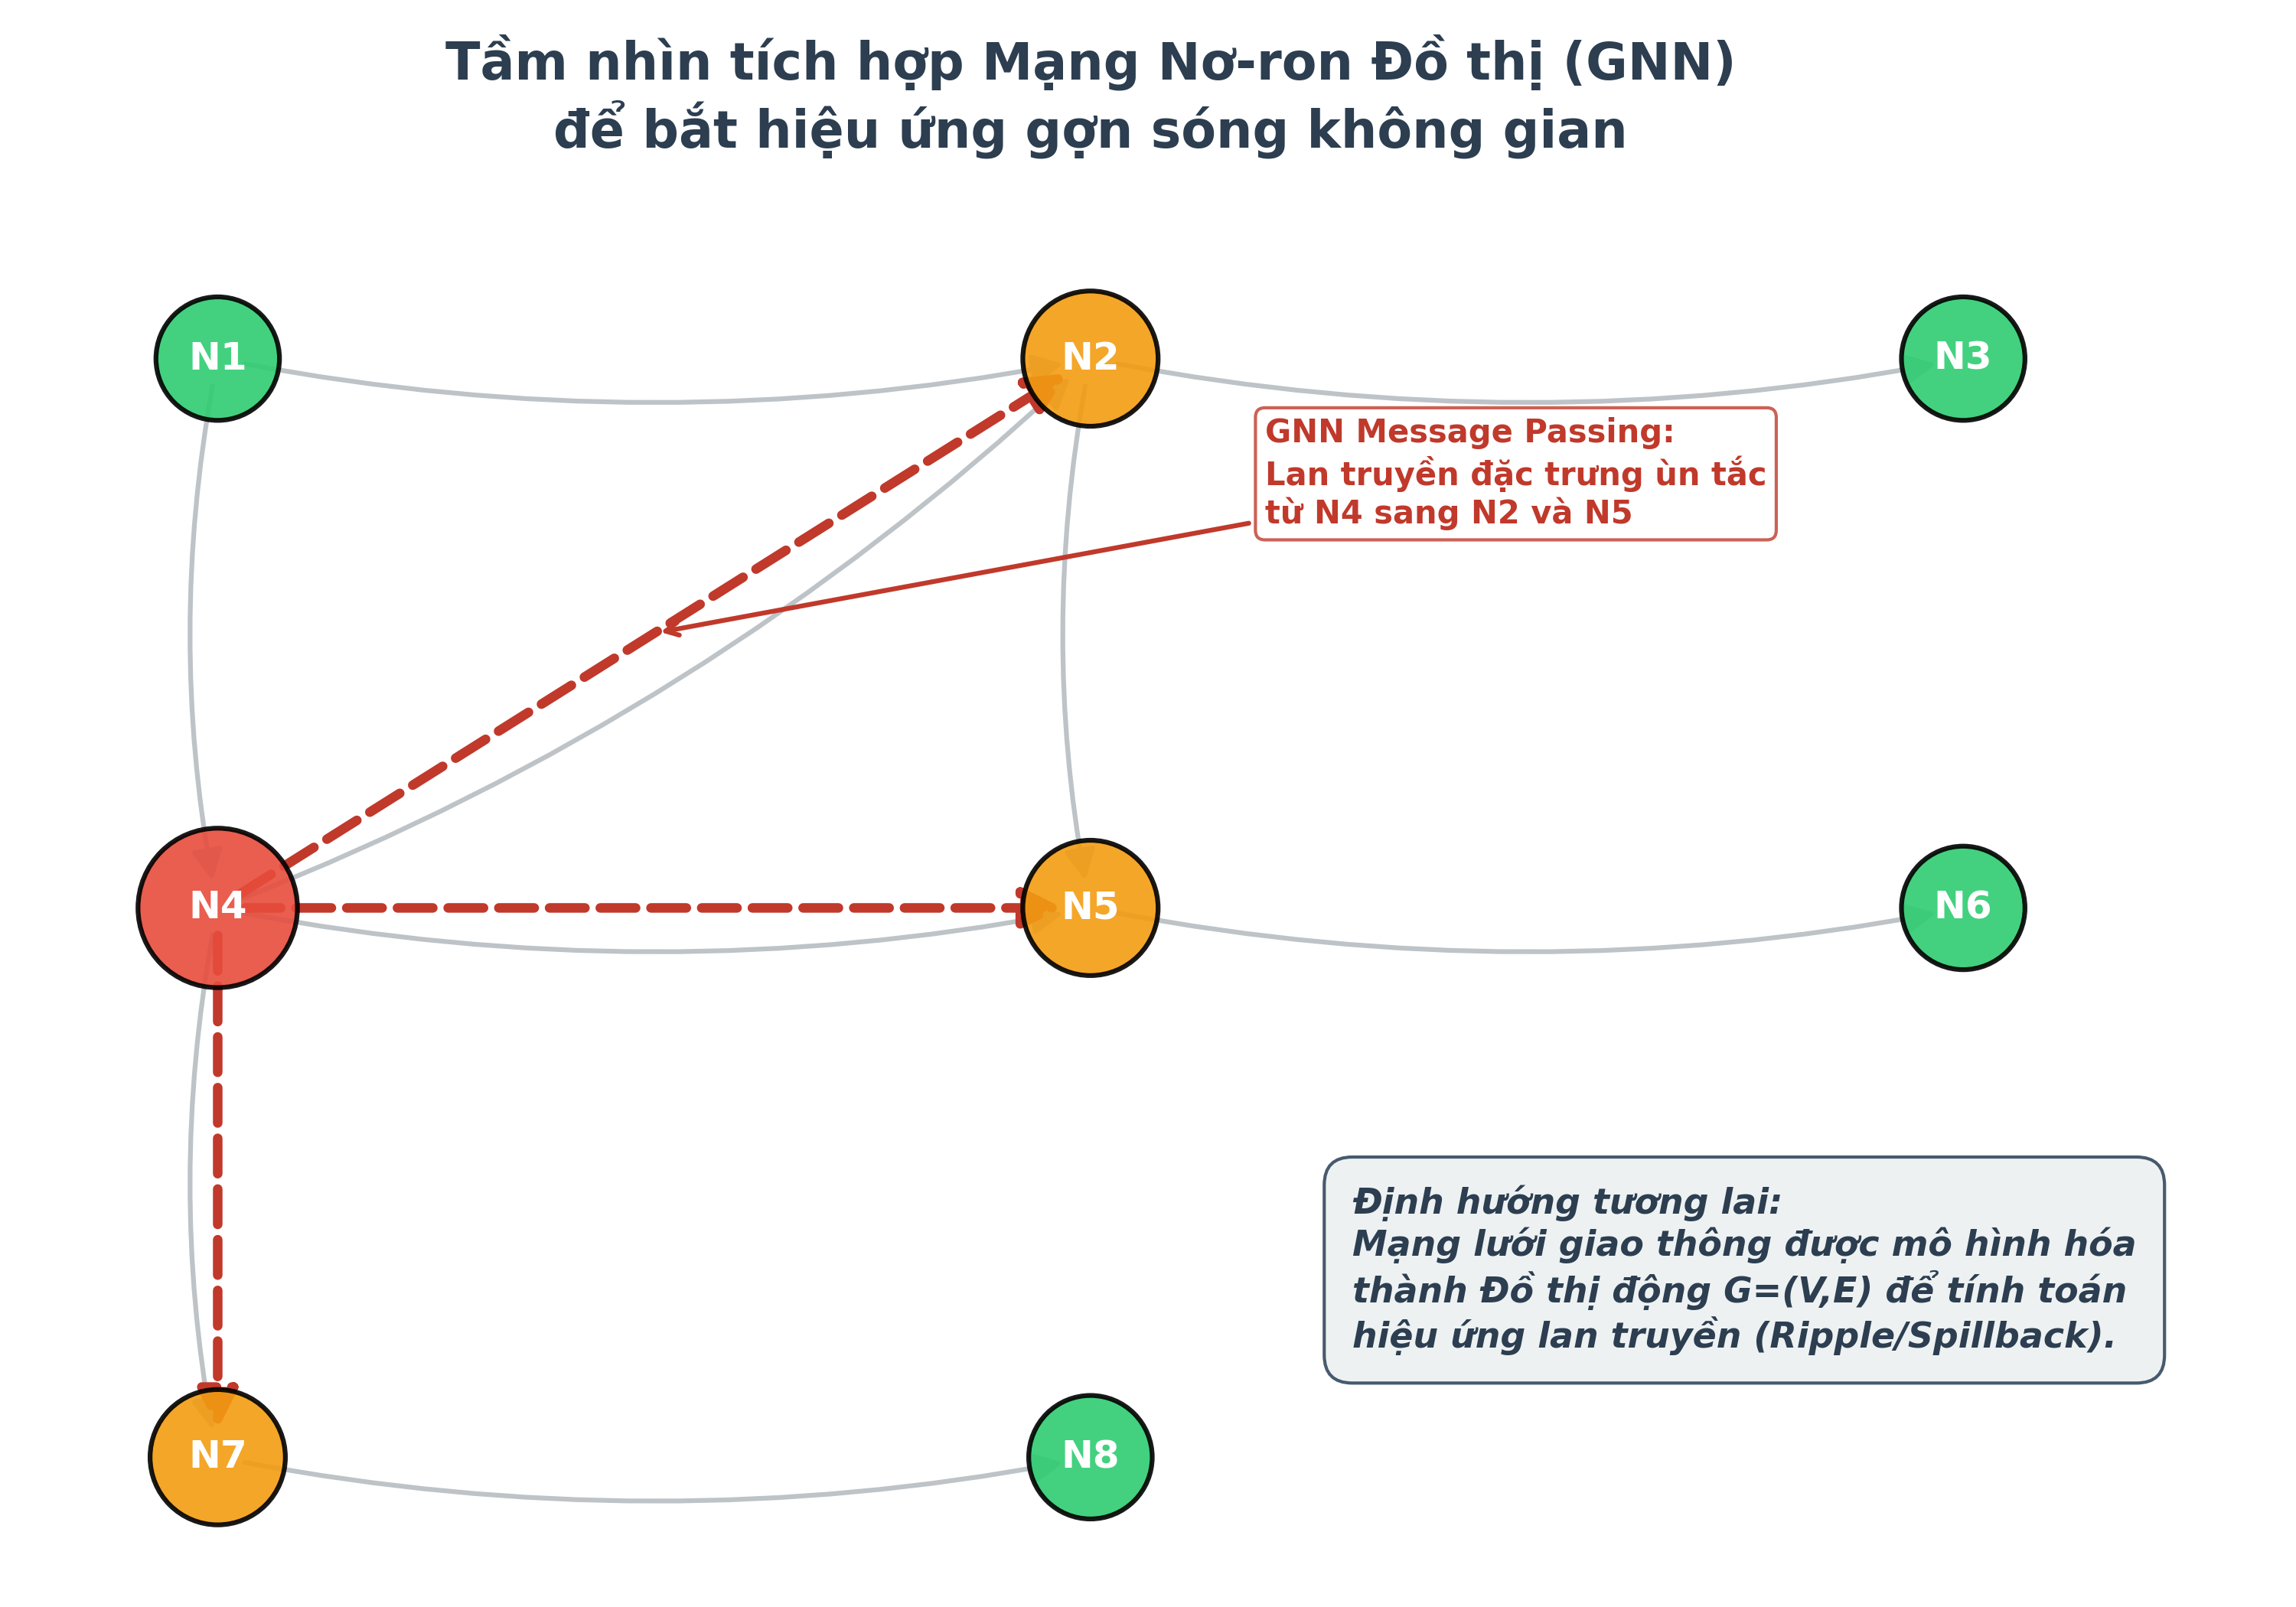
\includegraphics[width=0.8\textwidth]{Images/CH5/21.png}
    \vspace{12pt}
    \caption{Tích hợp Mạng Nơ-ron Đồ thị (GNN)}
    \label{fig:5_21}
\end{figure}
